% %%%%%%%%%%%%%%%%%%%%%%%%%%%%%%%%%%%%%%%%%%%%%%%%%%%%%%%%%%%
% \begin{frame}[fragile]\frametitle{}
% \begin{center}
% \Large{MidcurveNN : Encoder-Decoder Neural Network for Computing Midcurve of a Thin Polygon}
% \end{center}
% \end{frame}

%%%%%%%%%%%%%%%%%%%%%%%%%%%%%%%%%%%%%%%%%%%%%%%%%%%%%%%%%%%%%%%%%%%%%%%%%%%%%%%%%%
\begin{frame}[fragile]\frametitle{}
\begin{center}
{\Large Introduction}
\end{center}
\end{frame}

%%%%%%%%%%%%%%%%%%%%%%%%%%%%%%%%%%%%%%%%%%%%%%%%%%%%%%%%%%%%%%%%%%%%%%%%%%%%%%%%%%
\begin{frame}[fragile]\frametitle{}
\begin{center}
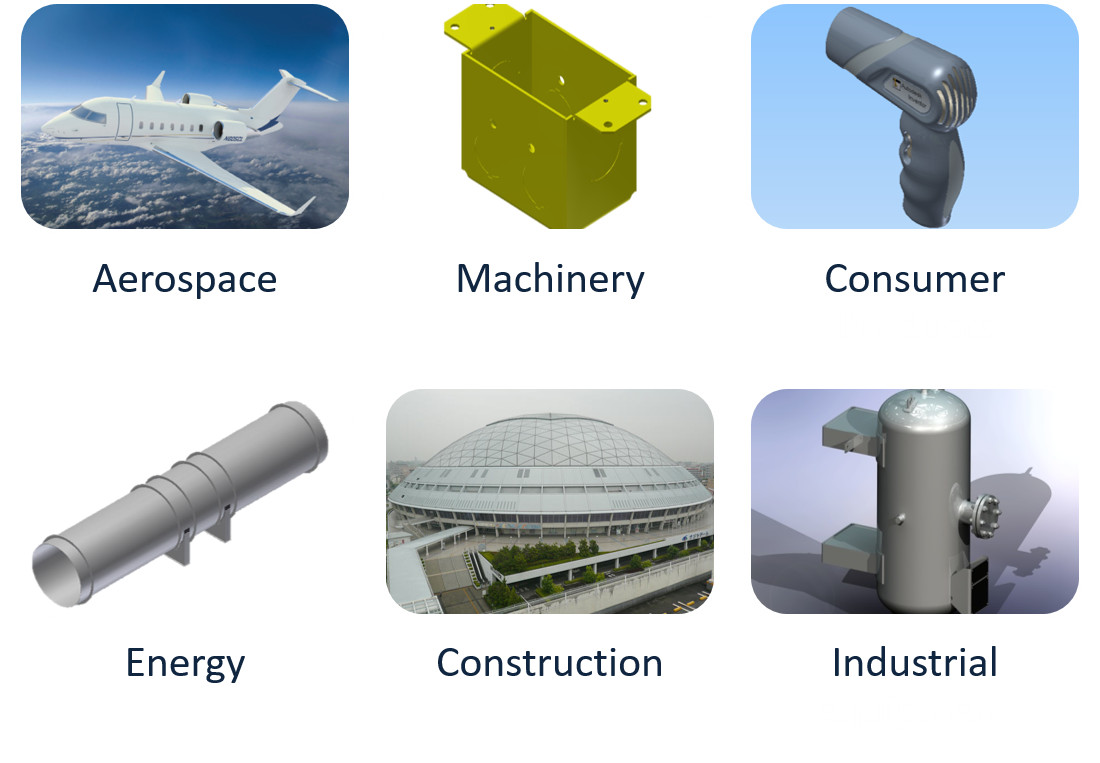
\includegraphics[width=0.9\linewidth,keepaspectratio]{midcurve1}
\end{center}
\end{frame}


%%%%%%%%%%%%%%%%%%%%%%%%%%%%%%%%%%%%%%%%%%%%%%%%%%%%%%%%%%%
\begin{frame}[fragile]\frametitle{Can we use shapes directly?}
	\begin{itemize}
	\item CAD : Designing Shapes
	\item CAE : Engineering Analysis
	\item CAD$\rightarrow$CAE: Simplification for quicker results.
	\end{itemize}

\begin{center}
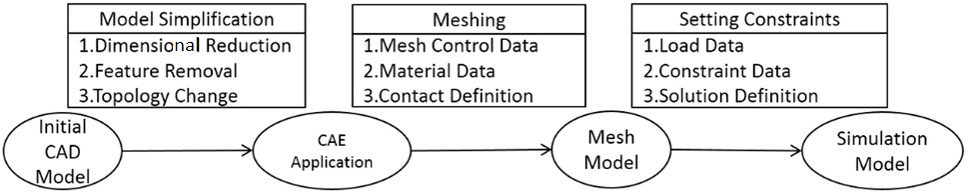
\includegraphics[width=\linewidth,keepaspectratio]{midcurve2}
\end{center}

\end{frame}

%%%%%%%%%%%%%%%%%%%%%%%%%%%%%%%%%%%%%%%%%%%%%%%%%%%%%%%%%%%%%%%%%%%%%%%%%%%%%%%%%%
\begin{frame}[fragile]\frametitle{CAD-CAE}
\begin{center}
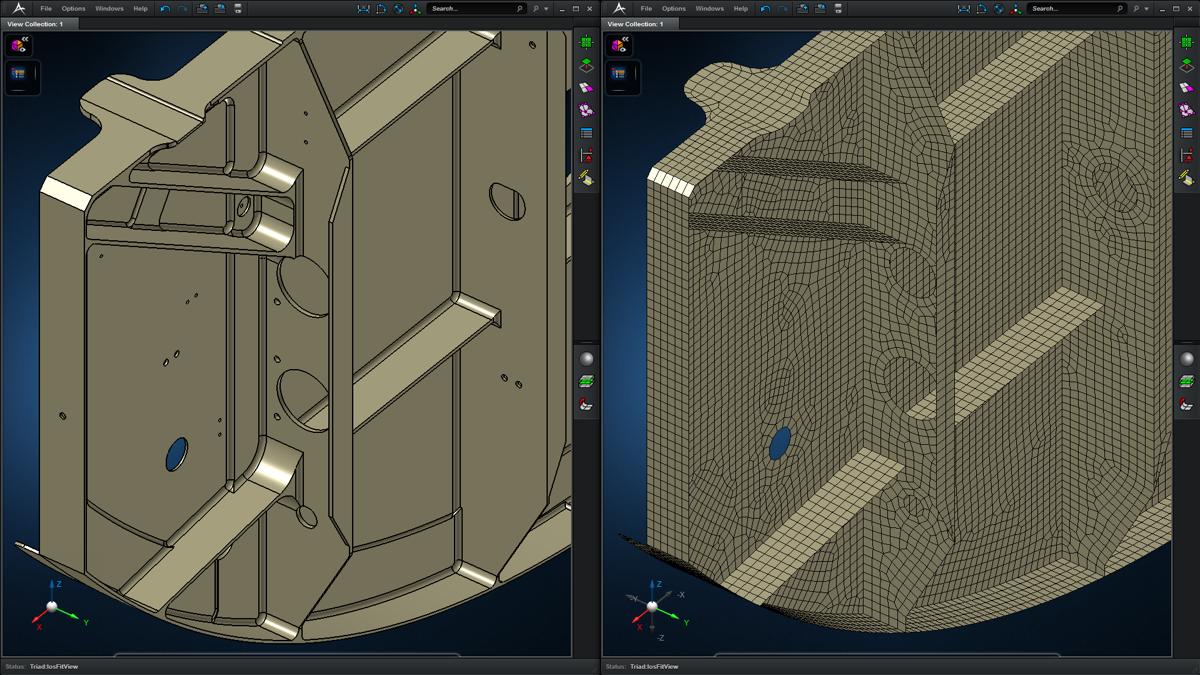
\includegraphics[width=0.9\linewidth,keepaspectratio]{midcurve3}
\end{center}
\end{frame}

%%%%%%%%%%%%%%%%%%%%%%%%%%%%%%%%%%%%%%%%%%%%%%%%%%%%%%%%%%%%%%%%%%%%%%%%%%%%%%%%%%
\begin{frame}[fragile]\frametitle{For Shapes like Sheet Metal \ldots}
\begin{center}
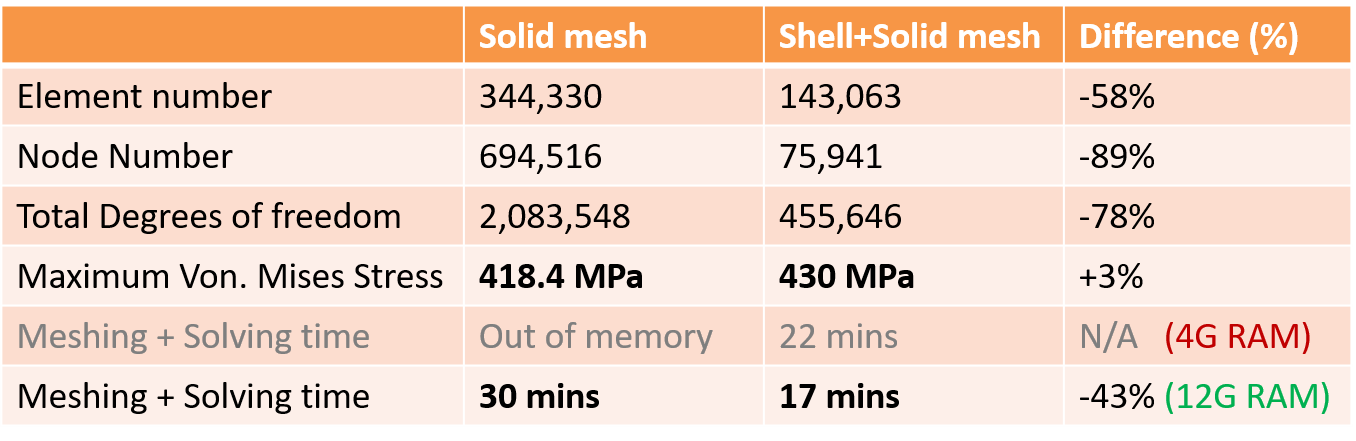
\includegraphics[width=\linewidth,keepaspectratio]{midcurve4}
\end{center}
Half the computation time, but similar accuracy
\end{frame}

%%%%%%%%%%%%%%%%%%%%%%%%%%%%%%%%%%%%%%%%%%%%%%%%%%%%%%%%%%%%%%%%%%%%%%%%%%%%%%%%%%
\begin{frame}[fragile]\frametitle{Midsurface is?}
\begin{center}
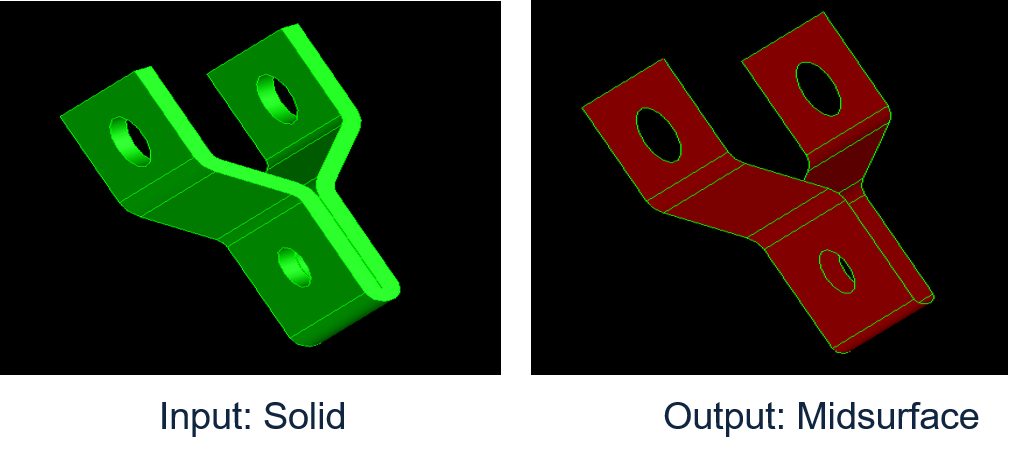
\includegraphics[width=0.9\linewidth,keepaspectratio]{midcurve5}
\end{center}
	\begin{itemize}
	\item Widely used for CAE of Thin-Walled parts
	\item Computation is challenging and still unsolved
	\end{itemize}
	
\end{frame}

%%%%%%%%%%%%%%%%%%%%%%%%%%%%%%%%%%%%%%%%%%%%%%%%%%%%%%%%%%%%%%%%%%%%%%%%%%%%%%%%%%
\begin{frame}[fragile]\frametitle{Getting Midsurface}

	\begin{itemize}
	\item Going on for decades \ldots
	\item Manually by offsetting and stitching, initially
	\item Many CAD-CAE packages give automatic option, but \ldots
	\end{itemize}
\begin{center}
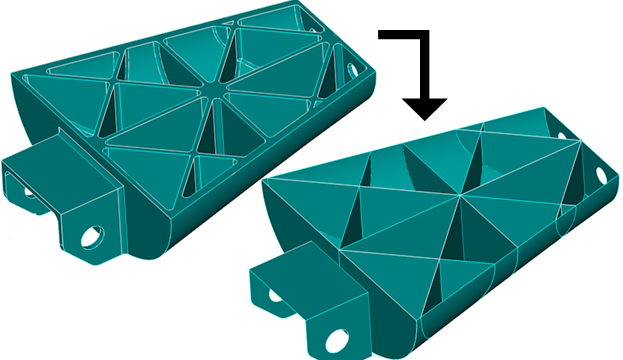
\includegraphics[width=0.8\linewidth,keepaspectratio]{midcurve6}
\end{center}	
\end{frame}

%%%%%%%%%%%%%%%%%%%%%%%%%%%%%%%%%%%%%%%%%%%%%%%%%%%%%%%%%%%%%%%%%%%%%%%%%%%%%%%%%%
\begin{frame}[fragile]\frametitle{Look at the output}
\begin{center}
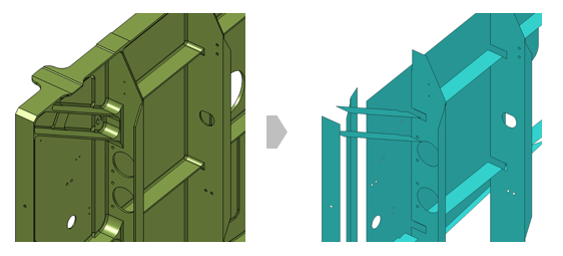
\includegraphics[width=\linewidth,keepaspectratio]{midcurve7}
\end{center}	
\end{frame}

%%%%%%%%%%%%%%%%%%%%%%%%%%%%%%%%%%%%%%%%%%%%%%%%%%%%%%%%%%%%%%%%%%%%%%%%%%%%%%%%%%
\begin{frame}[fragile]\frametitle{Can't tolerate gaps}

	\begin{itemize}
	\item We have thickness sampling, 
	\item To recreate-represent the original shape
	\item Input and output difference not desirable
	\end{itemize}
\end{frame}

%%%%%%%%%%%%%%%%%%%%%%%%%%%%%%%%%%%%%%%%%%%%%%%%%%%%%%%%%%%%%%%%%%%%%%%%%%%%%%%%%%
\begin{frame}[fragile]\frametitle{For a simple model like}
\begin{center}
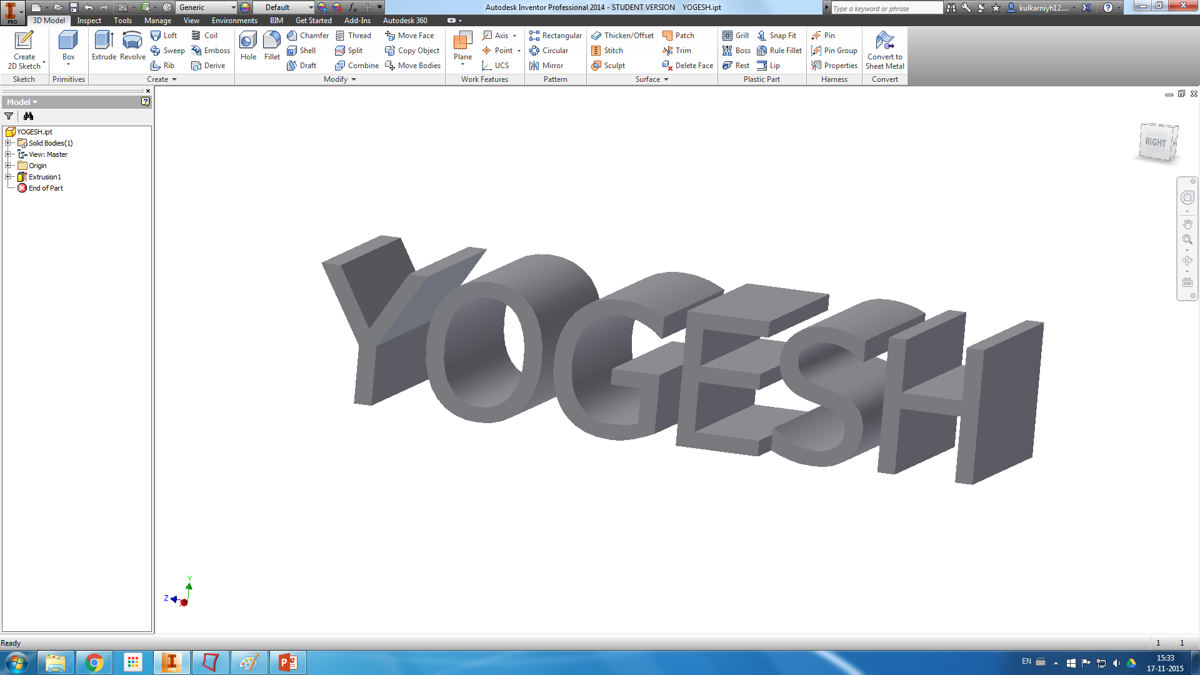
\includegraphics[width=0.9\linewidth,keepaspectratio]{midcurve8}
\end{center}	
\end{frame}

%%%%%%%%%%%%%%%%%%%%%%%%%%%%%%%%%%%%%%%%%%%%%%%%%%%%%%%%%%%%%%%%%%%%%%%%%%%%%%%%%%
\begin{frame}[fragile]\frametitle{You get}
\begin{center}
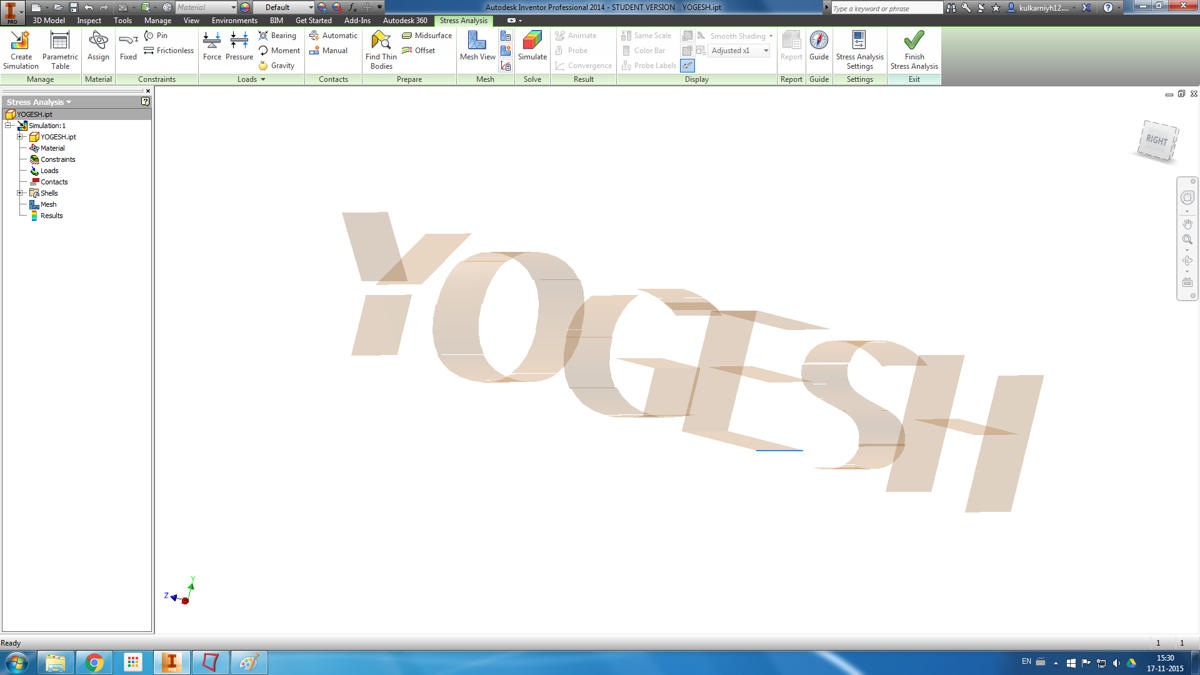
\includegraphics[width=0.9\linewidth,keepaspectratio]{midcurve9}
\end{center}	
\end{frame}

%%%%%%%%%%%%%%%%%%%%%%%%%%%%%%%%%%%%%%%%%%%%%%%%%%%%%%%%%%%%%%%%%%%%%%%%%%%%%%%%%%
\begin{frame}[fragile]\frametitle{For a far simpler shape}
\begin{center}
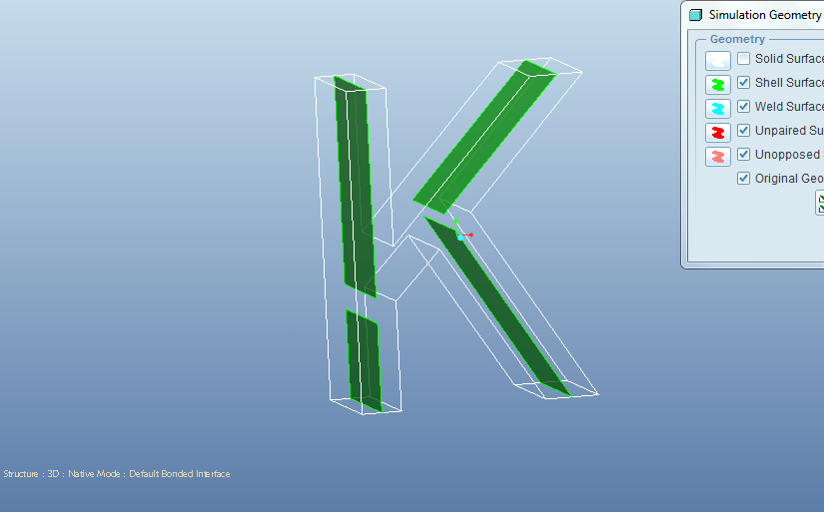
\includegraphics[width=0.9\linewidth,keepaspectratio]{midcurve10}
\end{center}	
\end{frame}

%%%%%%%%%%%%%%%%%%%%%%%%%%%%%%%%%%%%%%%%%%%%%%%%%%%%%%%%%%%%%%%%%%%%%%%%%%%%%%%%%%
\begin{frame}[fragile]\frametitle{Current Quality}
\begin{center}
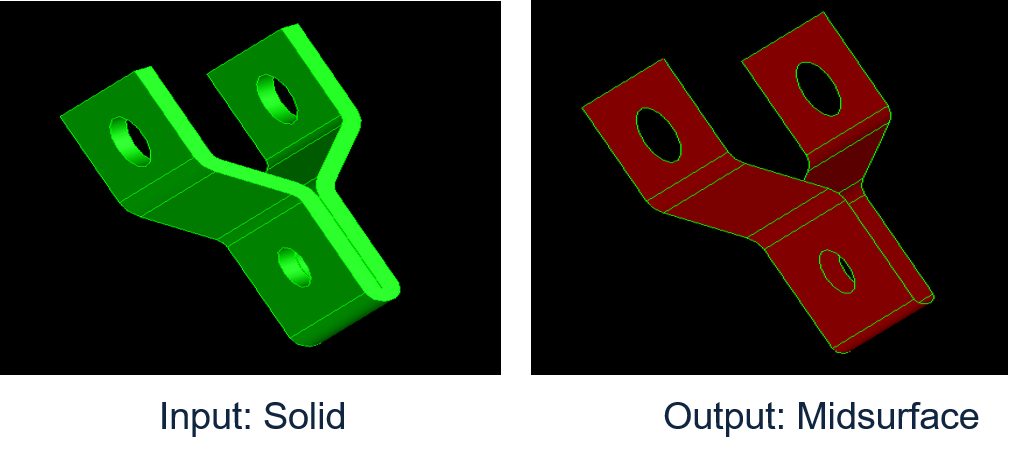
\includegraphics[width=0.9\linewidth,keepaspectratio]{midcurve5}
\end{center}
	\begin{itemize}
	\item Errors take weeks to correct for complex parts.
	\item But still preferred, due to vast savings time
	\item From Days to hours \ldots
	\end{itemize}
	
\end{frame}

%%%%%%%%%%%%%%%%%%%%%%%%%%%%%%%%%%%%%%%%%%%%%%%%%%%%%%%%%%%%%%%%%%%%%%%%%%%%%%%%%%
\begin{frame}[fragile]\frametitle{Midsurface Computation}

	\begin{itemize}
	\item Midsurface of a Patch is Midcurve of its profile extruded.
	\item So, it boils down to computing 1D midcurve of a 2D profile
	\end{itemize}
	
\begin{center}
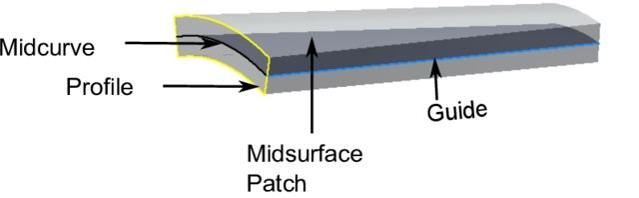
\includegraphics[width=0.9\linewidth,keepaspectratio]{midcurve12}
\end{center}	
\end{frame}

%%%%%%%%%%%%%%%%%%%%%%%%%%%%%%%%%%%%%%%%%%%%%%%%%%%%%%%%%%%%%%%%%%%%%%%%%%%%%%%%%%
\begin{frame}[fragile]\frametitle{What is a Midcurve?}

	\begin{itemize}
	\item Midsurface : From 3D thin Solid to 2D Surface
	\item Midcurve : From 2D Profile to 1D Curve
	\end{itemize}
	
\begin{center}
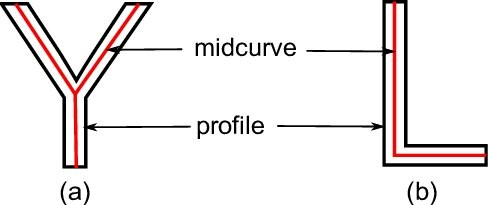
\includegraphics[width=0.6\linewidth,keepaspectratio]{midcurve13}
\end{center}	
\end{frame}

%%%%%%%%%%%%%%%%%%%%%%%%%%%%%%%%%%%%%%%%%%%%%%%%%%%%%%%%%%%%%%%%%%%%%%%%%%%%%%%%%%
\begin{frame}[fragile]\frametitle{Many Approaches}

	\begin{itemize}
	\item More than 6 decades of research…
	\item Most CAD-CAE packages…
	\item Rule-based!! Heuristic!! Case-by-case basis!!
	\end{itemize}
	
	
\begin{center}
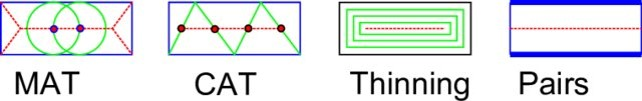
\includegraphics[width=0.9\linewidth,keepaspectratio]{midcurve14}
\end{center}	
\end{frame}

%%%%%%%%%%%%%%%%%%%%%%%%%%%%%%%%%%%%%%%%%%%%%%%%%%%%%%%%%%%%%%%%%%%%%%%%%%%%%%%%%%
\begin{frame}[fragile]\frametitle{When-What?}
\begin{center}
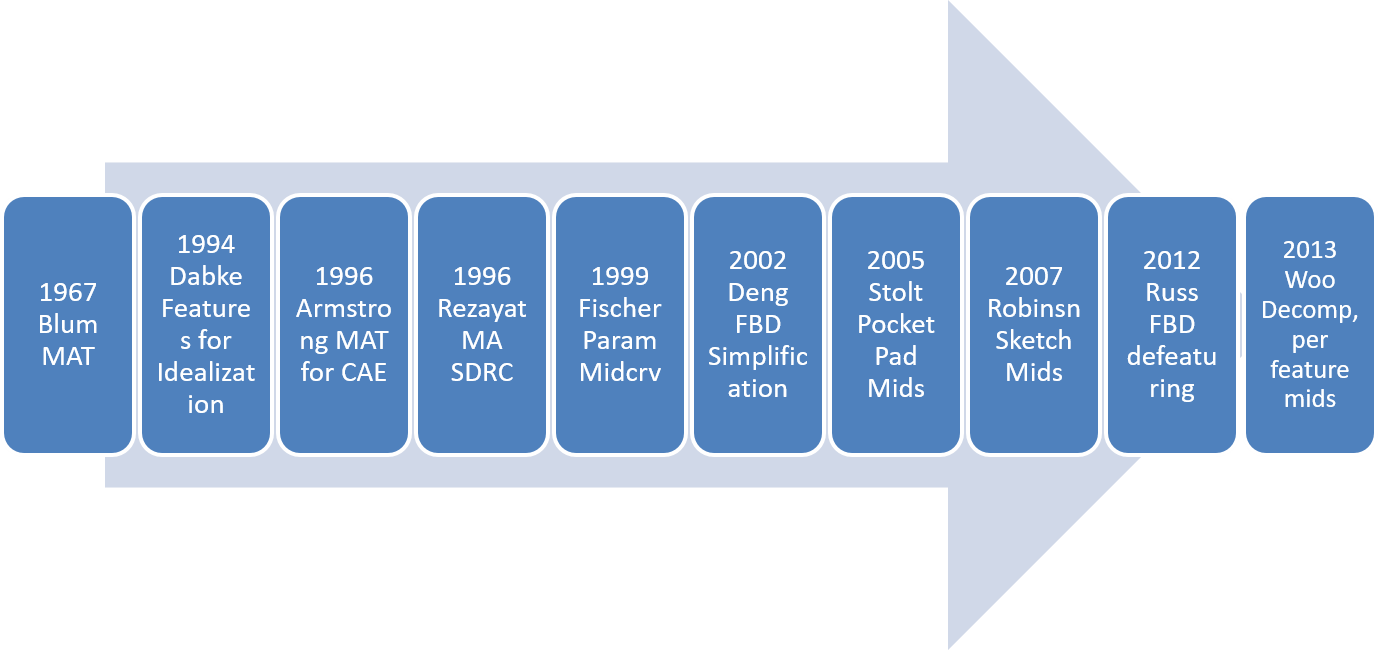
\includegraphics[width=\linewidth,keepaspectratio]{midcurve15}
\end{center}	
\end{frame}

%%%%%%%%%%%%%%%%%%%%%%%%%%%%%%%%%%%%%%%%%%%%%%%%%%%%%%%%%%%%%%%%%%%%%%%%%%%%%%%%%%
\begin{frame}[fragile]\frametitle{2017: My PhD Work: Rule-based}
\begin{center}
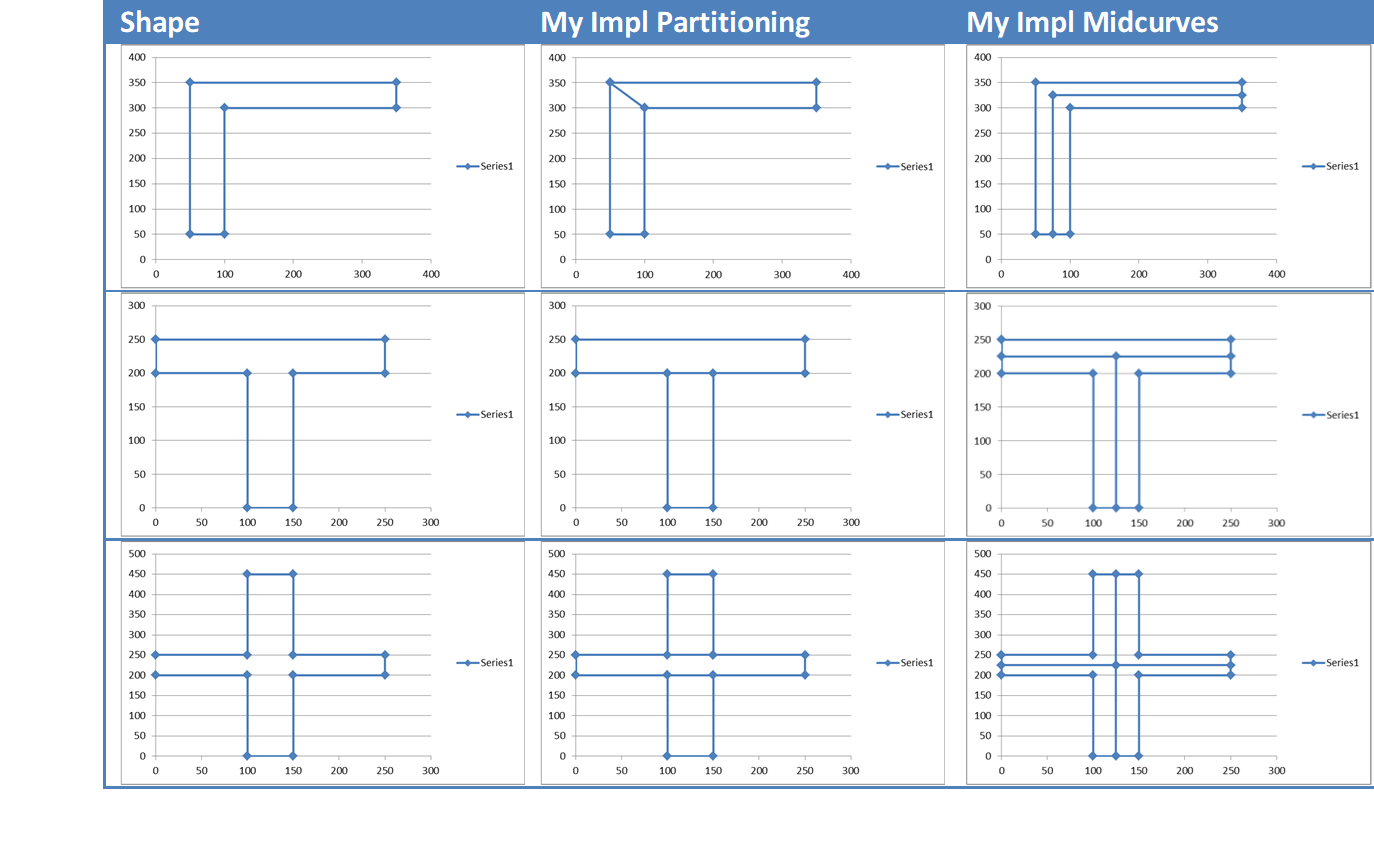
\includegraphics[width=\linewidth,keepaspectratio]{midcurve16}
\end{center}	
\end{frame}

%%%%%%%%%%%%%%%%%%%%%%%%%%%%%%%%%%%%%%%%%%%%%%%%%%%%%%%%%%%%%%%%%%%%%%%%%%%%%%%%%%
\begin{frame}[fragile]\frametitle{Limitations}

	\begin{itemize}
	\item Fully rule-based
	\item Need to adjust for new shapes
	\item So, not scalable
	\end{itemize}
\begin{center}

\includegraphics[width=0.3\linewidth,keepaspectratio]{midcurve17}
\end{center}	
\end{frame}

%%%%%%%%%%%%%%%%%%%%%%%%%%%%%%%%%%%%%%%%%%%%%%%%%%%%%%%%%%%%%%%%%%%%%%%%%%%%%%%%%%
\begin{frame}[fragile]\frametitle{Idea}
\begin{center}

\includegraphics[width=0.3\linewidth,keepaspectratio]{midcurve18}

Can Neural Networks ``learn'' the dimension reduction transformation?
\end{center}	
\end{frame}

%%%%%%%%%%%%%%%%%%%%%%%%%%%%%%%%%%%%%%%%%%%%%%%%%%%%%%%%%%%%%%%%%%%%%%%%%%%%%%%%%%
\begin{frame}[fragile]\frametitle{How?}

	\begin{itemize}
	\item Supply lots of training data of profiles and their corresponding midcurves and train.
	\item Then given an unseen profile, can Neural Network compute a midcurve, mimicking the original profile shape?
	\end{itemize}
\begin{center}

\includegraphics[width=0.3\linewidth,keepaspectratio]{midcurve18}
\end{center}	
\end{frame}

%%%%%%%%%%%%%%%%%%%%%%%%%%%%%%%%%%%%%%%%%%%%%%%%%%%%%%%%%%%%%%%%%%%%%%%%%%%%%%%%%%
\begin{frame}[fragile]\frametitle{Midcurve by Neural network}
\begin{center}
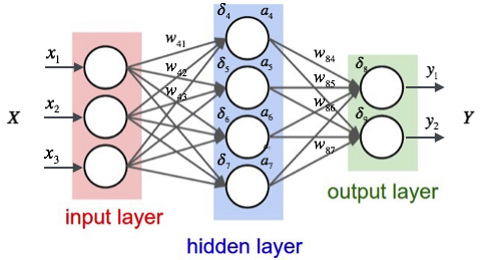
\includegraphics[width=\linewidth,keepaspectratio]{midcurve19}
\end{center}	
\end{frame}

%%%%%%%%%%%%%%%%%%%%%%%%%%%%%%%%%%%%%%%%%%%%%%%%%%%%%%%%%%%%%%%%%%%%%%%%%%%%%%%%%%
\begin{frame}[fragile]\frametitle{Midcurve : The Problem}

	\begin{itemize}
	\item {\bf Goal}: Given a 2D closed shape (closed polygon) find its midcurve (polyline, closed or open)
	\item {\bf Input}: set of points or set of connected lines, non-intersecting, simple, convex, closed polygon
	\item {\bf Output}: another set of points or set of connected lines, open/branched polygons possible
	\end{itemize}

\end{frame}

%%%%%%%%%%%%%%%%%%%%%%%%%%%%%%%%%%%%%%%%%%%%%%%%%%%%%%%%%%%%%%%%%%%%%%%%%%%%%%%%%%
\begin{frame}[fragile]\frametitle{Midcurve == Dimension Reduction}

	\begin{itemize}
	\item Like PCA (Principal Component Analysis), wish to find Principal curve
	\item That `represents' the original profile shape
	\end{itemize}
\begin{center}
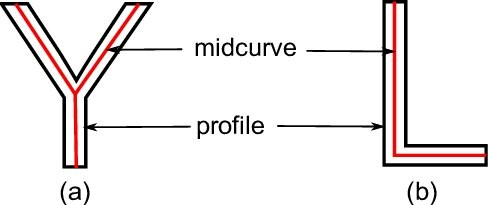
\includegraphics[width=0.6\linewidth,keepaspectratio]{midcurve20}
\end{center}	
\end{frame}

%%%%%%%%%%%%%%%%%%%%%%%%%%%%%%%%%%%%%%%%%%%%%%%%%%%%%%%%%%%%%%%%%%%%%%%%%%%%%%%%%%
\begin{frame}[fragile]\frametitle{Midcurve $==$ Translation}

	\begin{itemize}
	\item Left side (input): 2D Sketch Profile
	\item Right Side (output): 1D Midcurve
	\item Sequence 2 Sequence problem
	\end{itemize}
\begin{center}
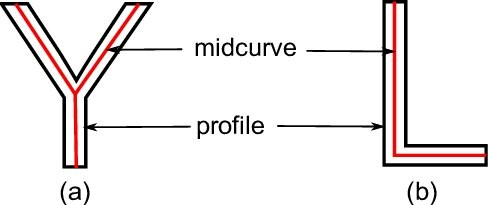
\includegraphics[width=0.6\linewidth,keepaspectratio]{midcurve20}
\end{center}	
\end{frame}

%%%%%%%%%%%%%%%%%%%%%%%%%%%%%%%%%%%%%%%%%%%%%%%%%%%%%%%%%%%%%%%%%%%%%%%%%%%%%%%%%%
\begin{frame}[fragile]\frametitle{Midcurve $!=$ Auto-Encoder Decoder}

	\begin{itemize}
	\item Its not Auto-Encoder as Input and Output are different
	\item Its not fixed size i/o as Input and Output sizes are different
	\end{itemize}
\begin{center}
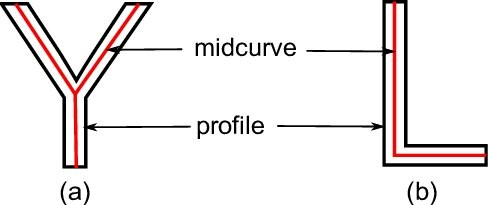
\includegraphics[width=0.6\linewidth,keepaspectratio]{midcurve20}
\end{center}	
\end{frame}

%%%%%%%%%%%%%%%%%%%%%%%%%%%%%%%%%%%%%%%%%%%%%%%%%%%%%%%%%%%%%%%%%%%%%%%%%%%%%%%%%%
\begin{frame}[fragile]\frametitle{Variable Size Encoder Decoder}

	\begin{itemize}
	\item Batches need fixed lengths
	\item Made fixed size by Padding.
	\end{itemize}
\begin{center}
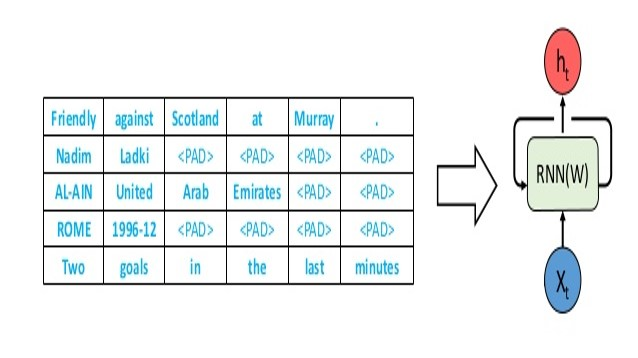
\includegraphics[width=\linewidth,keepaspectratio]{midcurve21}
\end{center}	
\end{frame}

%%%%%%%%%%%%%%%%%%%%%%%%%%%%%%%%%%%%%%%%%%%%%%%%%%%%%%%%%%%%%%%%%%%%%%%%%%%%%%%%%%
\begin{frame}[fragile]\frametitle{Variable Size Encoder Decoder}

	\begin{itemize}
	\item OK for NLP, say Machine Translations, where padding values like ``-1'' can be added along with other words (vectors or indices)
	\item But in Geometry, its not OK. 
	\item Because any value can represent a Valid Input, even though we don’t want it to be the input.
	\end{itemize}
	
\end{frame}

%%%%%%%%%%%%%%%%%%%%%%%%%%%%%%%%%%%%%%%%%%%%%%%%%%%%%%%%%%%%%%%%%%%%%%%%%%%%%%%%%%
\begin{frame}[fragile]\frametitle{A Twist to the problem}

  \begin{columns}[t]
    \begin{column}[T]{0.4\linewidth}
      \centering
      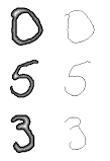
\includegraphics[width=0.9\linewidth,keepaspectratio]{midcurve22}
    \end{column}
    \begin{column}[T]{0.6\linewidth}
	\begin{itemize}
	\item Till we get good variable size encoder decoder network for geometry…
	\item Decided to convert this Sequence 2 Sequence problem as Image 2 Image problem.
	\end{itemize}
    \end{column}
  \end{columns}
  \end{frame}
  
%%%%%%%%%%%%%%%%%%%%%%%%%%%%%%%%%%%%%%%%%%%%%%%%%%%%%%%%%%%%%%%%%%%%%%%%%%%%%%%%%%
\begin{frame}[fragile]\frametitle{A Twist to the problem}

	\begin{itemize}
	\item Input: Black \& White Image of 2D profile
	\item Output: Black \& White Image of 1D midcurve
	\end{itemize}
\begin{center}
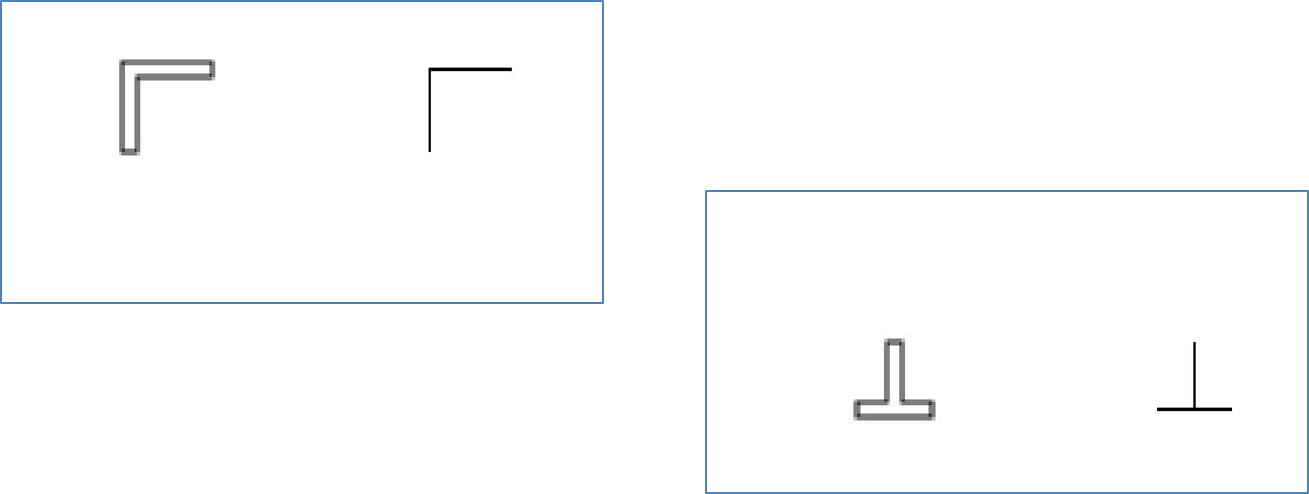
\includegraphics[width=0.9\linewidth,keepaspectratio]{midcurve23}
\end{center}	
\end{frame}

%%%%%%%%%%%%%%%%%%%%%%%%%%%%%%%%%%%%%%%%%%%%%%%%%%%%%%%%%%%%%%%%%%%%%%%%%%%%%%%%%%
\begin{frame}[fragile]\frametitle{Solves \ldots}
Problems of Geometric sequences

	\begin{itemize}
	\item Variable input/output sizes
	\item Loops need to be crossed
	\item Branches
	\end{itemize}
\begin{center}
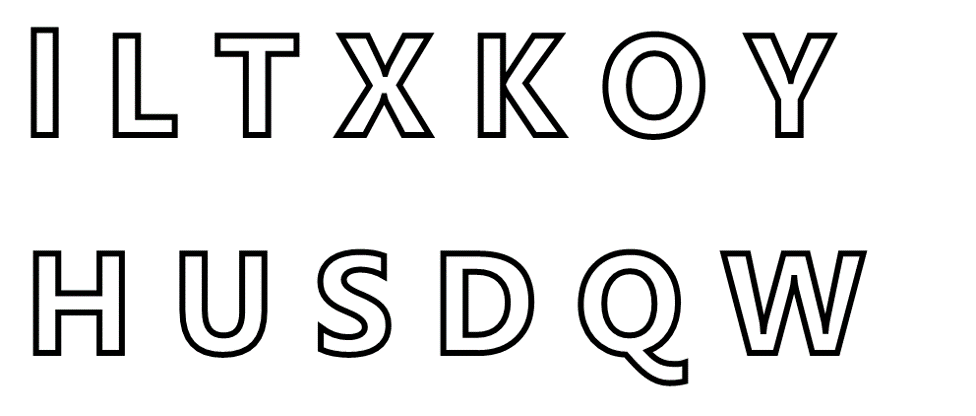
\includegraphics[width=0.9\linewidth,keepaspectratio]{midcurve24}
\end{center}	
\end{frame}

%%%%%%%%%%%%%%%%%%%%%%%%%%%%%%%%%%%%%%%%%%%%%%%%%%%%%%%%%%%%%%%%%%%%%%%%%%%%%%%%%%
\begin{frame}[fragile]\frametitle{Reuse Image Encoder Decoder}
\begin{center}
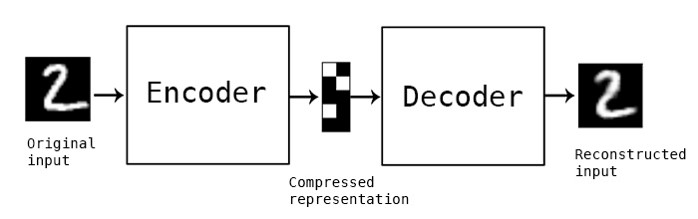
\includegraphics[width=0.9\linewidth,keepaspectratio]{midcurve25}
\end{center}	
\end{frame}

%%%%%%%%%%%%%%%%%%%%%%%%%%%%%%%%%%%%%%%%%%%%%%%%%%%%%%%%%%%%%%%%%%%%%%%%%%%%%%%%%%
\begin{frame}[fragile]\frametitle{For Dimension Reduction}
\begin{center}
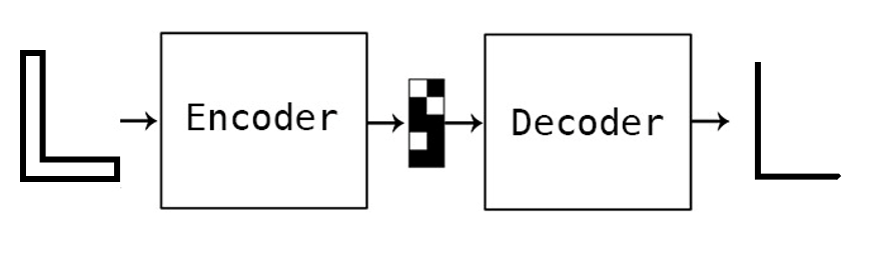
\includegraphics[width=0.9\linewidth,keepaspectratio]{midcurve26}
\end{center}	
\end{frame}

%%%%%%%%%%%%%%%%%%%%%%%%%%%%%%%%%%%%%%%%%%%%%%%%%%%%%%%%%%%%%%%%%%%%%%%%%%%%%%%%%%
\begin{frame}[fragile]\frametitle{For Deep Learning}
	\begin{itemize}
	\item Need lots of data
	\item Had just few input output image pairs
	\item How to augment/populate large variations \ldots
	\end{itemize}
\end{frame}

%%%%%%%%%%%%%%%%%%%%%%%%%%%%%%%%%%%%%%%%%%%%%%%%%%%%%%%%%%%%%%%%%%%%%%%%%%%%%%%%%%
\begin{frame}[fragile]\frametitle{}
\begin{center}
{\Large Data Preparation}
\end{center}
\end{frame}

%%%%%%%%%%%%%%%%%%%%%%%%%%%%%%%%%%%%%%%%%%%%%%%%%%%%%%%%%%%%%%%%%%%%%%%%%%%%%%%%%%
\begin{frame}[fragile]\frametitle{Data}

Original input and output are in the form of polylines, meaning a list of points, each having x,y coordinates

\begin{center}
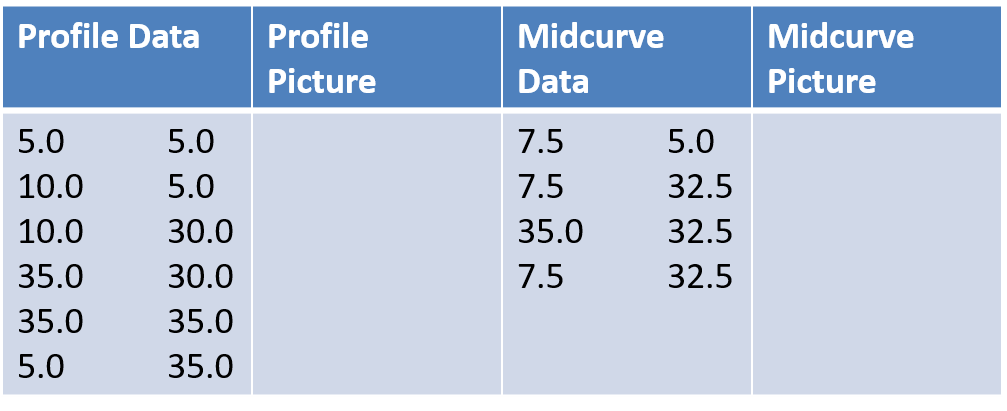
\includegraphics[width=0.9\linewidth,keepaspectratio]{midcurve27}
\end{center}	
\end{frame}

%%%%%%%%%%%%%%%%%%%%%%%%%%%%%%%%%%%%%%%%%%%%%%%%%%%%%%%%%%%%%%%%%%%%%%%%%%%%%%%%%%
\begin{frame}[fragile]\frametitle{Data}
\begin{center}
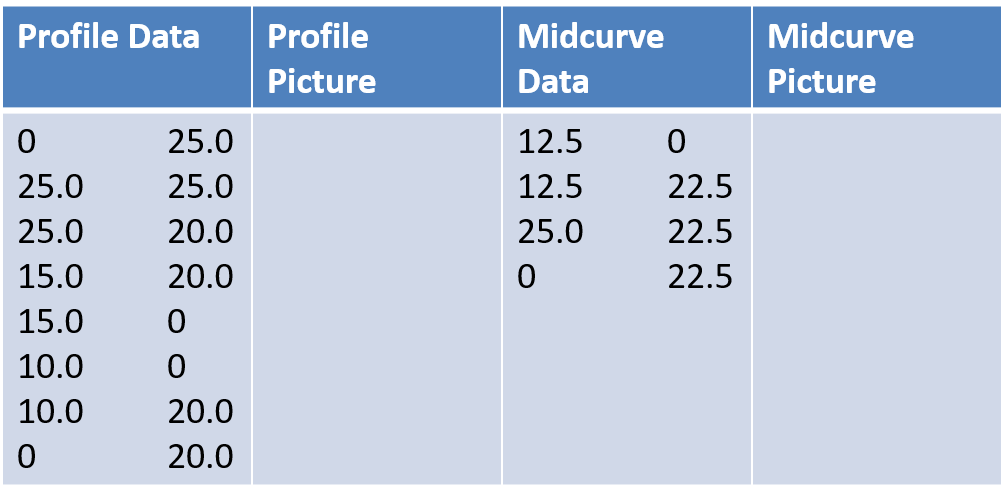
\includegraphics[width=0.9\linewidth,keepaspectratio]{midcurve28}
\end{center}

	\begin{itemize}
	\item For each shape, we have this pair of input and output. That's it. 
	\item We need to start with these few samples only
	\end{itemize}
	
\end{frame}

%%%%%%%%%%%%%%%%%%%%%%%%%%%%%%%%%%%%%%%%%%%%%%%%%%%%%%%%%%%%%%%%%%%%%%%%%%%%%%%%%%
\begin{frame}[fragile]\frametitle{Augmentation}

	\begin{itemize}
	\item Such few profile shapes, are  just not enough for Neural Networks to train.
	\item Need more with as much diversity as possible.
	\item Will need to artificially augment data with transformations, like pan, rotate, mirror, etc.
	\item All needs to be automatically, programmatically
	\end{itemize}
	
\end{frame}

%%%%%%%%%%%%%%%%%%%%%%%%%%%%%%%%%%%%%%%%%%%%%%%%%%%%%%%%%%%%%%%%%%%%%%%%%%%%%%%%%%
\begin{frame}[fragile]\frametitle{Geometry to Image}
	\begin{itemize}
	\item Raw input data is in the Vector format
	\item Converted it to fixed size $(100x100)$ image by rasterization of drawSVG library.
	\end{itemize}
\begin{center}
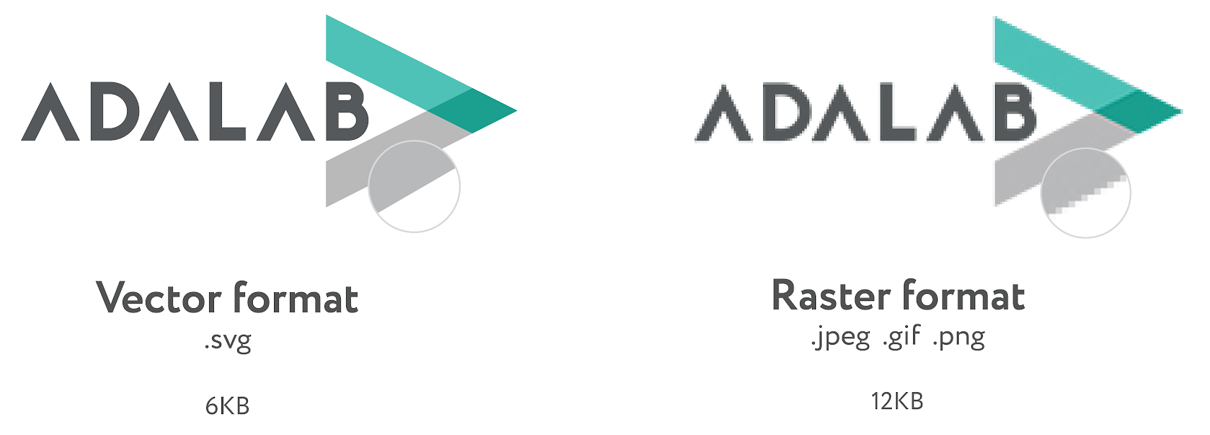
\includegraphics[width=0.9\linewidth,keepaspectratio]{midcurve29}
\end{center}	
\end{frame}

%%%%%%%%%%%%%%%%%%%%%%%%%%%%%%%%%%%%%%%%%%%%%%%%%%%%%%%%%%%%%%%%%%%%%%%%%%%%%%%%%%
\begin{frame}[fragile]\frametitle{Variations}

  \begin{columns}[t]
    \begin{column}[T]{0.4\linewidth}
      \centering
      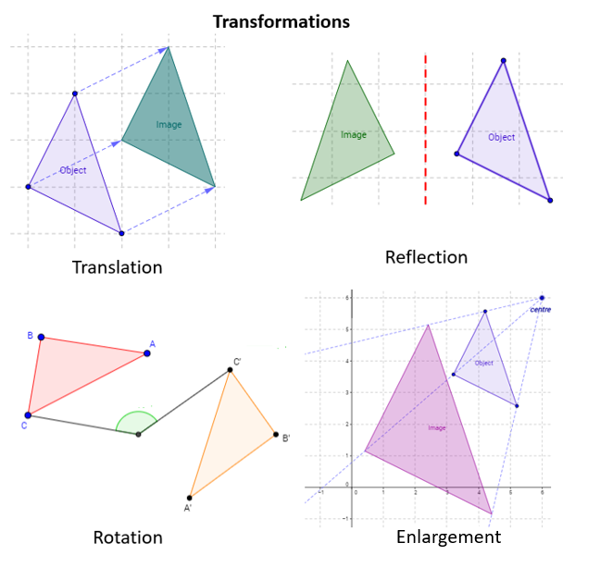
\includegraphics[width=0.9\linewidth,keepaspectratio]{midcurve30}
    \end{column}
    \begin{column}[T]{0.6\linewidth}
	\begin{itemize}
	\item Inputs: I, L, Plus, T
	\item Operations:
	\begin{itemize}
		\item Translated
		\item Rotated
		\item Mirrored
		\item Mirrored Translated
		\item Mirrored Rotated
	\end{itemize}
	\item Total: 896 images (still less, but not bad)
	\end{itemize}
    \end{column}
  \end{columns}
  \end{frame}
  
 %%%%%%%%%%%%%%%%%%%%%%%%%%%%%%%%%%%%%%%%%%%%%%%%%%%%%%%%%%%%%%%%%%%%%%%%%%%%%%%%%%
\begin{frame}[fragile]\frametitle{Training Data Samples}

\begin{center}
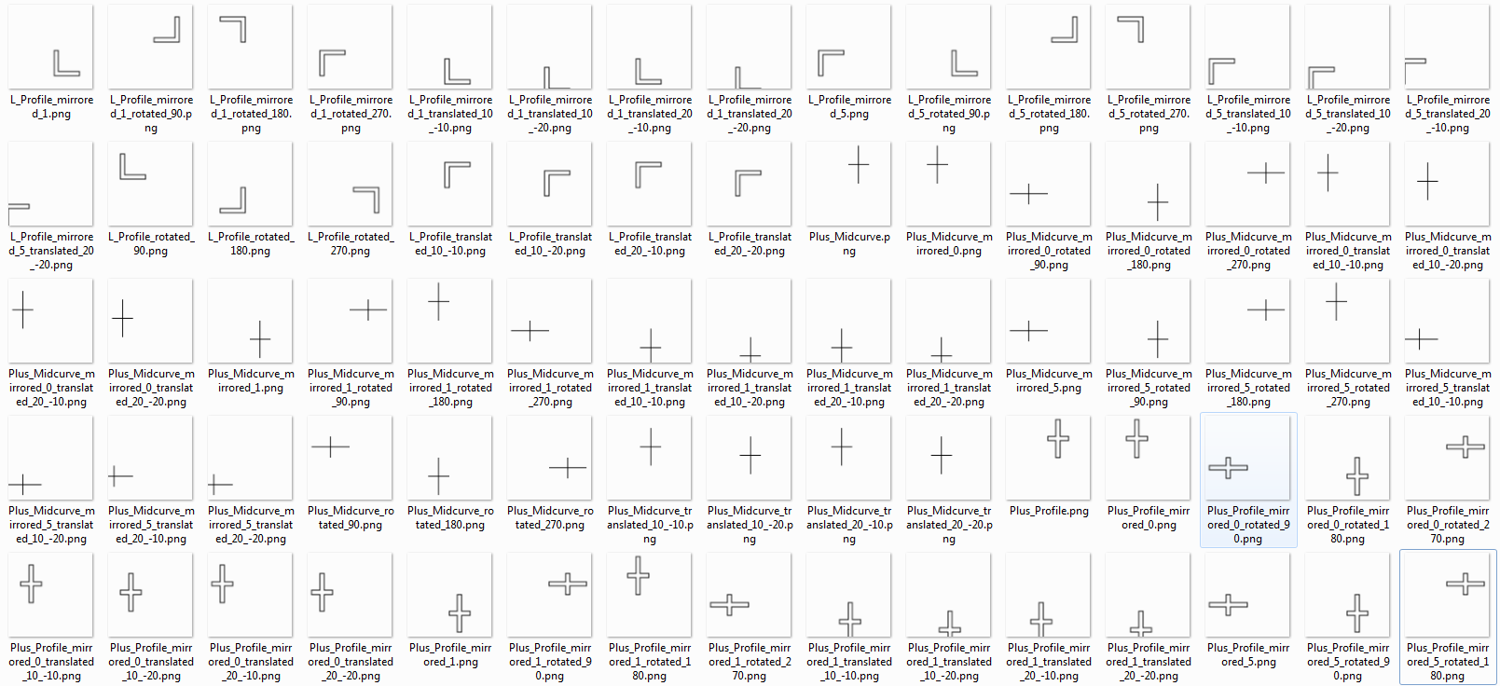
\includegraphics[width=\linewidth,keepaspectratio]{midcurve31}
\end{center}	
\end{frame}

%%%%%%%%%%%%%%%%%%%%%%%%%%%%%%%%%%%%%%%%%%%%%%%%%%%%%%%%%%%%%%%%%%%%%%%%%%%%%%%%%%
\begin{frame}[fragile]\frametitle{}
\begin{center}
{\Large Midcurve By Neural Network}
\end{center}
\end{frame}

%%%%%%%%%%%%%%%%%%%%%%%%%%%%%%%%%%%%%%%%%%%%%%%%%%%%%%%%%%%%%%%%%%%%%%%%%%%%%%%%%%
\begin{frame}[fragile]\frametitle{Options For Architectures}
	\begin{itemize}
	\item Simple Encoder Decoder (one layer each)
	\item Dense Encoder Decoder
	\item Convolutional Encoder Decoder
	\item Pix2Pix
	\item \ldots
	\end{itemize}	
\end{frame}

%%%%%%%%%%%%%%%%%%%%%%%%%%%%%%%%%%%%%%%%%%%%%%%%%%%%%%%%%%%%%%%%%%%%%%%%%%%%%%%%%%
\begin{frame}[fragile]\frametitle{}
\begin{center}
{\Large Simple Encoder Decoder}
\end{center}
\end{frame}

%%%%%%%%%%%%%%%%%%%%%%%%%%%%%%%%%%%%%%%%%%%%%%%%%%%%%%%%%%%%%%%%%%%%%%%%%%%%%%%%%%
\begin{frame}[fragile]\frametitle{Simple Encoder Decoder}

\begin{center}
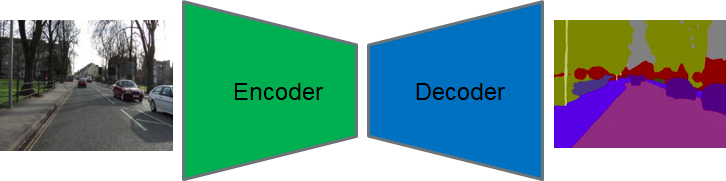
\includegraphics[width=0.9\linewidth,keepaspectratio]{midcurve32}
\end{center}	
\end{frame}

%%%%%%%%%%%%%%%%%%%%%%%%%%%%%%%%%%%%%%%%%%%%%%%%%%%%%%%%%%%%%%%%%%%%%%%%%%%%%%%%%%
\begin{frame}[fragile]\frametitle{Keras Implementation}

\begin{lstlisting}
input_img = Input(shape=(input_dim,))
    
encoded = Dense(encoding_dim, activation='relu',activity_regularizer=regularizers.l1(10e-5))(input_img)
decoded = Dense(input_dim, activation='sigmoid')(encoded) 
    
autoencoder = Model(input_img, decoded)
            
encoder = Model(input_img, encoded)
encoded_input = Input(shape=(encoding_dim,))
decoder_layer = autoencoder.layers[-1]
decoder = Model(encoded_input, decoder_layer(encoded_input))
    
autoencoder.compile(optimizer='adadelta', loss='binary_crossentropy')
\end{lstlisting}	
\end{frame}

%%%%%%%%%%%%%%%%%%%%%%%%%%%%%%%%%%%%%%%%%%%%%%%%%%%%%%%%%%%%%%%%%%%%%%%%%%%%%%%%%%
\begin{frame}[fragile]\frametitle{Results}

\begin{center}
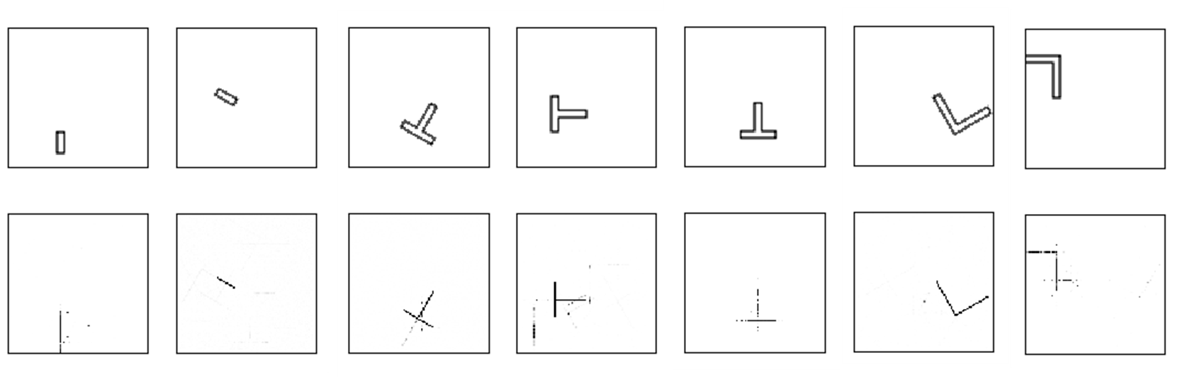
\includegraphics[width=\linewidth,keepaspectratio]{midcurve33}
\end{center}	
\end{frame}

%%%%%%%%%%%%%%%%%%%%%%%%%%%%%%%%%%%%%%%%%%%%%%%%%%%%%%%%%%%%%%%%%%%%%%%%%%%%%%%%%%
\begin{frame}[fragile]\frametitle{Results}
	\begin{itemize}
	\item Not very perfect but encouraging
	\item NN is correct with 
	\begin{itemize}
	\item The location (bounding box)
	\item Dimension Reduction is seen
	\end{itemize}	
	\item But, still some stray points and misses
	\end{itemize}	
\end{frame}

%%%%%%%%%%%%%%%%%%%%%%%%%%%%%%%%%%%%%%%%%%%%%%%%%%%%%%%%%%%%%%%%%%%%%%%%%%%%%%%%%%
\begin{frame}[fragile]\frametitle{What can be done?}
	\begin{itemize}
	\item For the noise, use bounding boxes 
	\item Feedback into error term: differencing with the known output expected 
	\item Classify single pixel image as the skeleton, and rest as noise. 
	\end{itemize}	
\end{frame}

%%%%%%%%%%%%%%%%%%%%%%%%%%%%%%%%%%%%%%%%%%%%%%%%%%%%%%%%%%%%%%%%%%%%%%%%%%%%%%%%%%
\begin{frame}[fragile]\frametitle{What Next?}
	\begin{itemize}
	\item Add denoiser network after the current one
	\item More Network Architectures
	\item Sequence-to-Sequence based approaches, taking closed thin polygon as input and polyline as output
	\item Extending to 3D, ie Midsurface
	\end{itemize}	
\end{frame}

%%%%%%%%%%%%%%%%%%%%%%%%%%%%%%%%%%%%%%%%%%%%%%%%%%%%%%%%%%%%%%%%%%%%%%%%%%%%%%%%%%
\begin{frame}[fragile]\frametitle{}
\begin{center}
{\Large End Notes}
\end{center}
\end{frame}


%%%%%%%%%%%%%%%%%%%%%%%%%%%%%%%%%%%%%%%%%%%%%%%%%%%%%%%%%%%%%%%%%%%%%%%%%%%%%%%%%%
\begin{frame}[fragile]\frametitle{Summary}
	\begin{itemize}
	\item Various applications need lower dimensional representation of shapes. 
	\item Midcurve is one- dimensional(1D) representation of a two-dimensional (2D) planar shape. 
	\item Used in animation, shape matching, retrieval, finite element analysis, etc. 
	\end{itemize}	
\end{frame}

%%%%%%%%%%%%%%%%%%%%%%%%%%%%%%%%%%%%%%%%%%%%%%%%%%%%%%%%%%%%%%%%%%%%%%%%%%%%%%%%%%
\begin{frame}[fragile]\frametitle{Summary}
	\begin{itemize}
	\item Approaches: Thinning, Medial Axis Transform (MAT), Chordal Axis Transform (CAT), Straight Skeletons, etc., all of which are rule-based.
	\item Proposing a novel method called MidcurveNN which uses Encoder-Decoder neural network for computing midcurve from images of 2D thin polygons in supervised learning manner. 
	\end{itemize}	
\end{frame}

%%%%%%%%%%%%%%%%%%%%%%%%%%%%%%%%%%%%%%%%%%%%%%%%%%%%%%%%%%%%%%%%%%%%%%%%%%%%%%%%%%
\begin{frame}[fragile]\frametitle{Summary}
	\begin{itemize}
	\item This dimension reduction transformation from input 2D thin polygon image to output 1D midcurve image is learnt by the neural network,
	\item Which can then be used to compute midcurve of an unseen 2D thin polygonal shape.
	\end{itemize}	
\end{frame}